\section{Additional Experiments}
\label{app:qwen}

Here, we reproduce similar trends from the main text on the Qwen3 model family, demonstrating that our results and algorithms are model and dataset agnostic. 

\begin{figure}[ht]
    \centering
    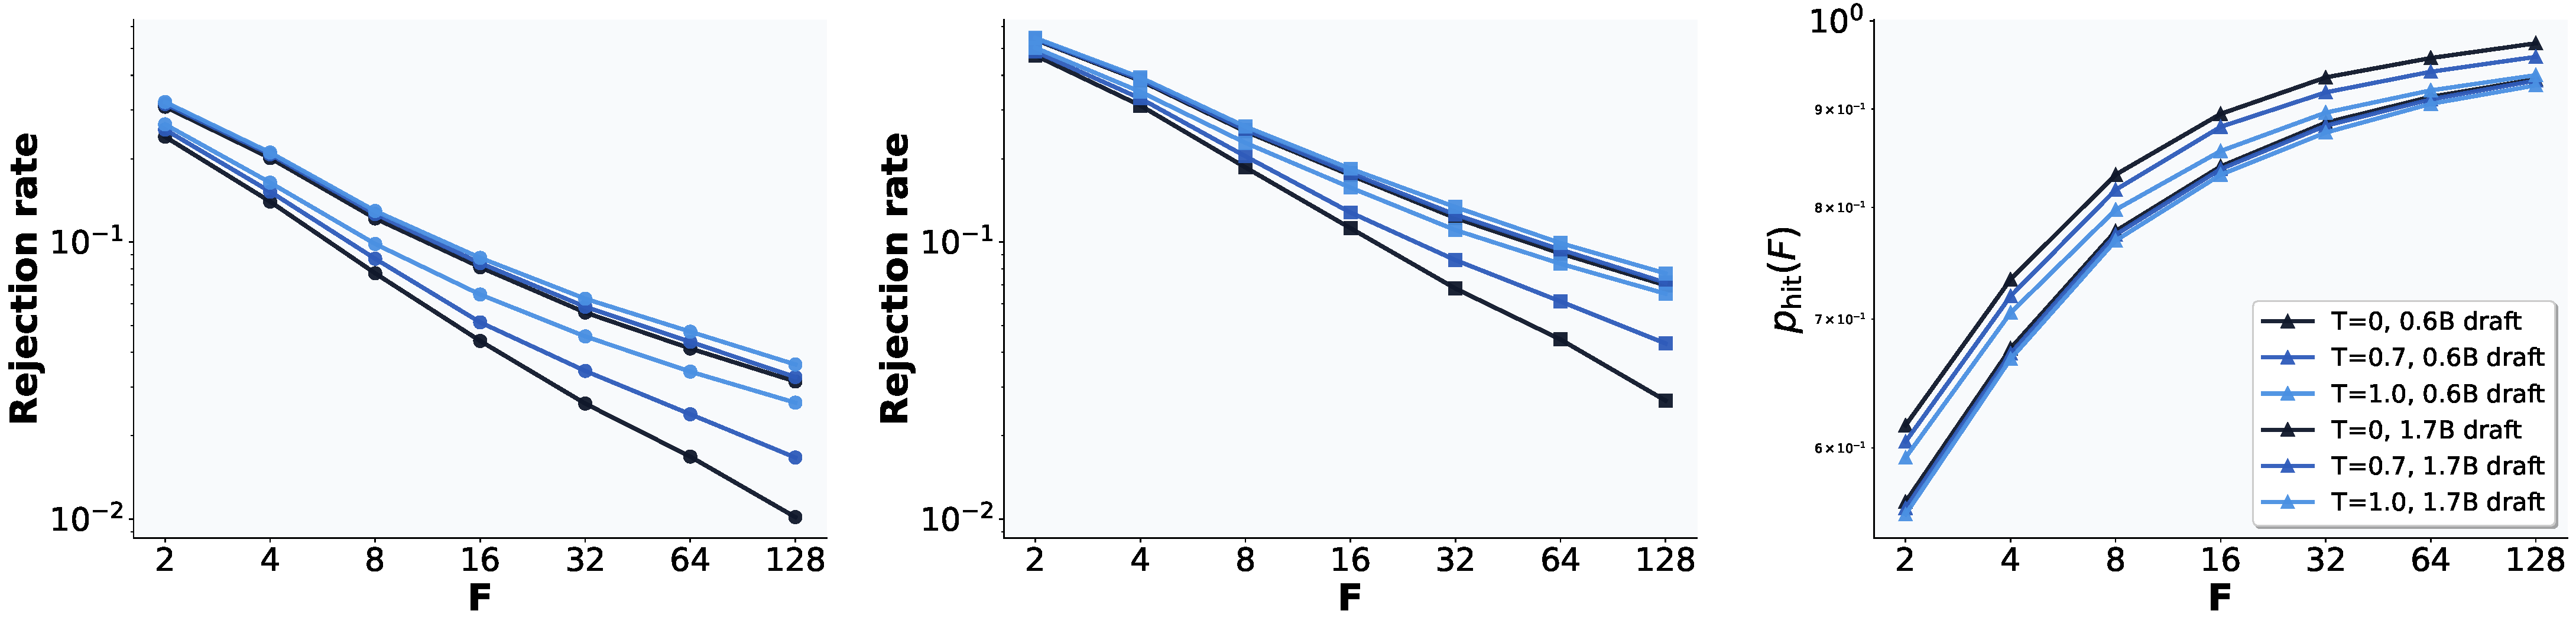
\includegraphics[width=\linewidth]{figures/dts_analysis_T0_T0.7_T1.0_0.6B_1.7B_target32B_loglog_reject.pdf}
    \caption{Rejection rate and cache hit rate scaling for Qwen-3 model family. Like the Llama-3 model family, we see it is an approximate power law in the fan-out, so that cache hit rates increase steadily as we grow $F$, the size of our cache.}
    \label{fig:dts-qwen}
\end{figure}

\begin{figure}[ht]
    \centering
    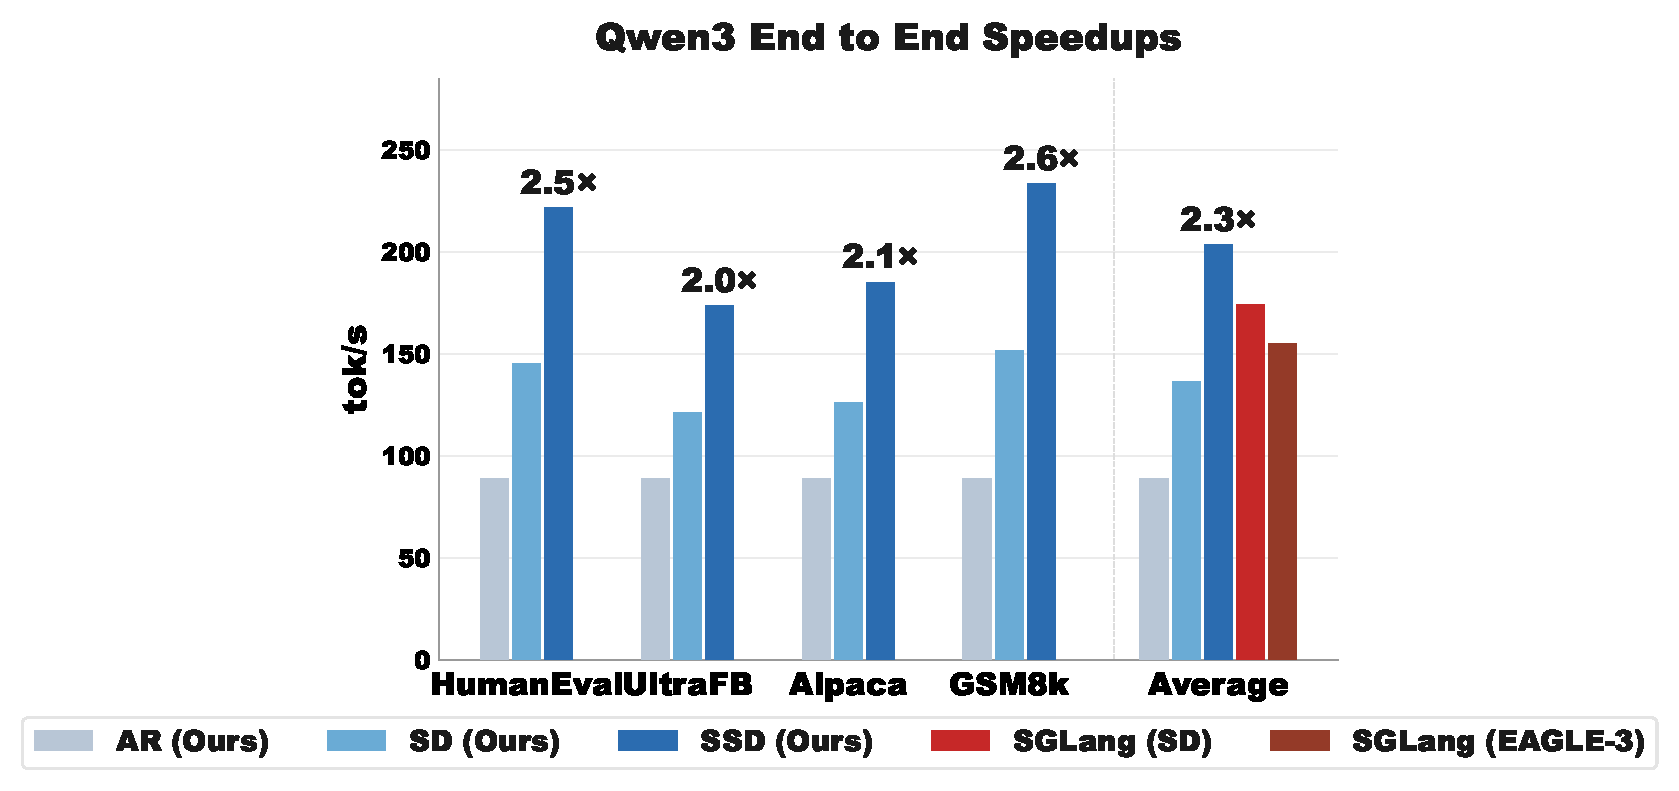
\includegraphics[width=\linewidth]{figures/qwen_e2e.pdf}
    \caption{End-to-end decoding speed comparison of SSD compared to SD and standard autoregressive decoding on Qwen-3 32B across four datasets.}
    \label{fig:e2e-qwen}
\end{figure}

\begin{figure}[ht]
    \centering
    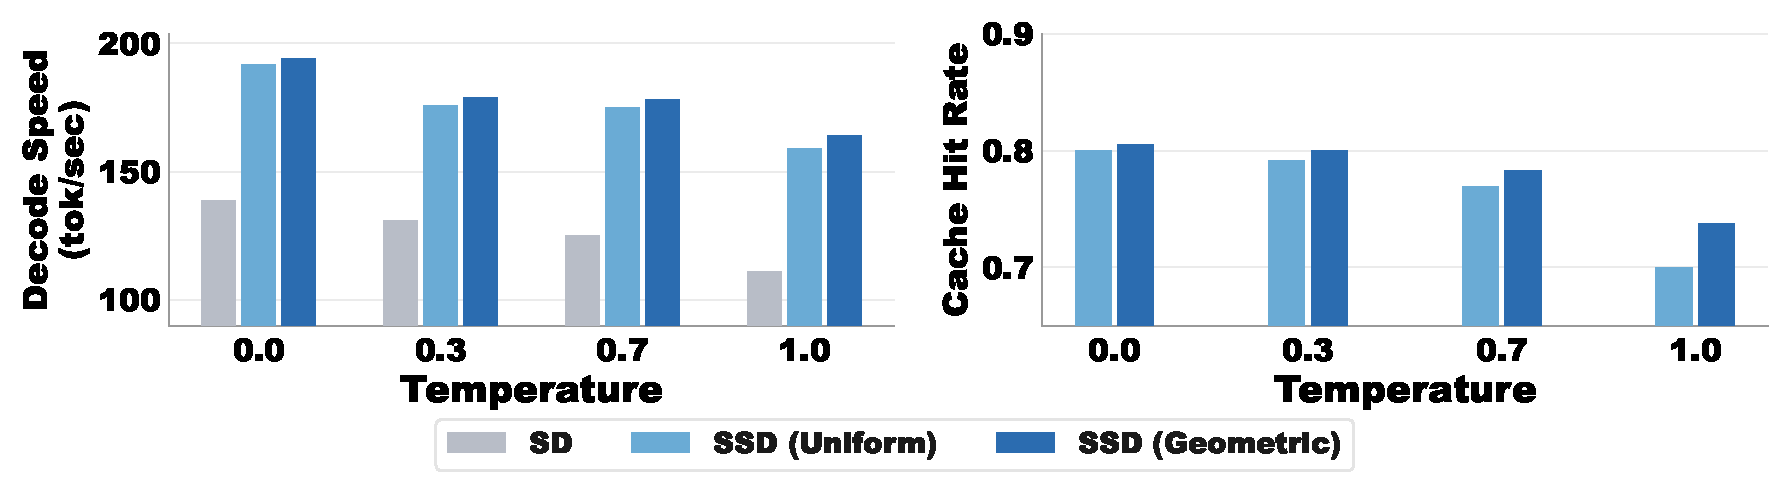
\includegraphics[width=\linewidth]{figures/temp_fan_out_qwen.pdf}
    \caption{End-to-end speed for Qwen-3 model family compared to synchronous baselines.}
    \label{fig:temp-fanout-qwen}
\end{figure}

\begin{figure}[ht]
    \centering
    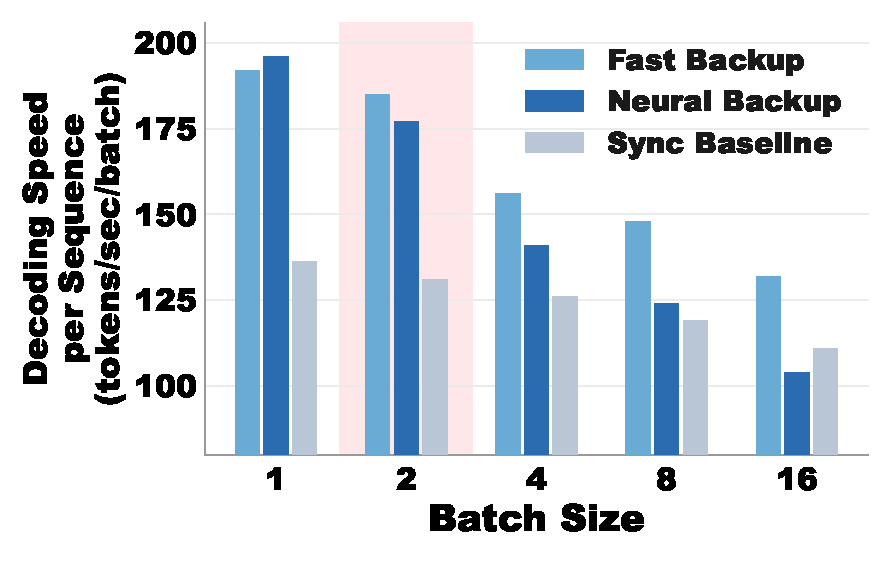
\includegraphics[width=0.7\linewidth]{figures/batch_scaling_qwen.pdf}
    \caption{Batch size scaling of Qwen-3 models compared to synchronous baselines.}
    \label{fig:qwen3-bsz}
\end{figure}